\documentclass{article}
\usepackage[utf8]{inputenc}
\usepackage{romannum}
\usepackage{amsfonts}
\usepackage{amssymb}
\usepackage{fancyhdr}
\usepackage{graphicx}
\usepackage{t1enc}
\usepackage{pdfpages}
\usepackage[magyar]{babel}
\usepackage[utf8]{inputenc}
\usepackage{amsmath}
\usepackage{mathtools}
\usepackage{pdfpages}
\usepackage{ marvosym } 
\usepackage{wrapfig}
\usepackage{hyperref}
\usepackage{pgfplots}

\pgfplotsset{width=\textwidth,compat=newest}
\hypersetup{
    colorlinks,
    citecolor=black,
    filecolor=black,
    linkcolor=black,
    urlcolor=black
}
\usepackage{romannum}
\usepackage{amsfonts}
\usepackage{amssymb}
\usepackage{fancyhdr}
\usepackage{graphicx}
\usepackage{t1enc}
\usepackage{svg}
\usepackage{listings}
\usepackage[magyar]{babel}
\usepackage[left=2cm,right=2cm,top=2cm,bottom=2cm]{geometry}

\title{K+F Projekt dokumentáció}
\author{}
\date{2}
\pagestyle{fancy}
\lhead{K+F Projekt dokumentáció}
\rhead{\includegraphics[scale=0.15]{acsg.png}}
\cfoot{\thepage. oldal}

\begin{document}
\pagenumbering{arabic}

\begin{center}
    \hrule
    \vspace{0.5cm}
    \begin{Huge}
    K+F projekt dokumentáció\\
    ACSG Kft.\\
    \end{Huge}
    \vspace{0.5cm}
    \begin{huge}
    Időszak:\\
    \end{huge}
    \begin{Large}
    2022.09.01. - 2022.10.31.\\
    \end{Large} \vspace{10pt}
    \begin{large}
    Készítette: Wenesz Dominik\\
    \end{large}\vspace{0.5cm}
    \hrule
    
  \end{center}
  \begin{figure}[b]
      \centering
      \includegraphics[]{acsg.png}
  \end{figure}
  


\thispagestyle{empty}
\setcounter{page}{0}




\newpage
\tableofcontents
\newpage

\section{Összefoglaló}
Az specifikált időintervallumban a kutatásfejlesztési projekt keretén belüli
előrehaladásokat, eredményeket, konklúziókat ezen dokumentumban, illetőleg
1-3 hónapos periódusokra lebontva hasonló tematikai felépítéssel kerülnek dokumentálásra.\\
Ezen beszámolók rövid összefoglalót tartalmaznak, a részletes leírás az egyes
részegységek folyamatosan bővülő dokumentációjában található meg, ezen egységek
a következők:
\begin{itemize}
    \item Objektum detektáló alrendszer
    \item Manipulátor alrendszer
    \item Optimalizációs alrendszer
    \item Biztonsági alrendszer
    \item Grafikus interfész
\end{itemize}
\textbf{2022.09.01. - 2022.10.31.:}\\
Az időszakon belül főként az \textbf{objektum detektáló alrendszer} elvi felépítésének,
alkalmazható algoritmusoknak, hardvereknek milyenségéről végeztünk kutatómunkát.\\
Továbbá az egyes algoritmusok implementálását, tesztelését is elkezdtük szoftveres
környezetben.\vspace{10pt}\\
A \textbf{manipulátor alrendszer} tekintetében egy SCARA robotra esett a választásunk, melynek
installálása megtörtént egy elzárt tesztkörnyezetben.\vspace{10pt}\\
Az \textbf{optimaliációs alrendszer} szempontjából érdemi előrehaladás nem történt az időszakban.\vspace{10pt}\\
A \textbf{biztonsági alrendszer} a SCARA robot üzembe helyezése közben a standard ipari robotoknál
szokásos részekkel ellátásra került, ezek a végleges rendszer esetében is ilyen formában
lesznek implementálva.\vspace{10pt}\\
A \textbf{grafikus interfészt} tekintve koncepcionális tervek születtek.

\section{Objektum detektáló alrendszer}
Az objektum detektáló alrendszer szempontjából a precizitás és sebesség a két fő aspektus,
melyek az esetek többségében együtt csak igen optimális esetben teljesülnek.\vspace{5pt}\\
\textbf{Hardver}\\
A kutatásfejlesztés során fontos figyelembe vennünk az egyes algoritmusok tesztelése,
összehasonlítása során a beágyazott rendszerek általi limitáltságot, hiszen nem lenne
optimális ha a képfeldolgozó rendszer mögött egy nagyteljesítményű PC-t üzemeltetni.\\
Egyrészt energetikai okokból, másrészt minden bizonnyal egy PC esetében az erőforrások
nem lennének teljesen kihasználva, másrészt stabilitási és integritásbeli problémákhoz
is vezethet, továbbá invesztálási költségben a tipikus beágyazttrendszerbeli hardverek
nagyságrendekkel olcsóbbak.\vspace{5pt}\\
Ennek megfelelően mivel a feladat számításigénye meglehetősen nagy, egyszerű mikrokontrollerek
nem alkalmazhatók, náluk nagyobb teljesítményű úgynevezett single board computer-eket 
tudunk képfeldolgozási célokra használni. Tekintve, hogy mesterséges intelligenciát is 
alkalmazni kívánunk valós időben, ezért fontos, hogy a számítások párhzamosan gyorsan
végrehajtásra kerüljenek, így megfelelő GPU-val rendelkező eszközre van szükségünk a projektben.\vspace{5pt}\\
Irodalomkutatás után hasonló alkalmazásokra tipikusan két modellt használnak:
\begin{itemize}
    \item RASPBERRY PI 4 MODEL B
    \item NVIDIA JETSON NANO
\end{itemize}
Számítási teljesítményben, memóriában és I/O tekintetében szinte teljesen megegyeznek 
egymással, azonban a Jetson Nano az NVIDIA kifejezetten mesterséges intelligencia és 
képfeldolgozáson alapuló applikációkra fejlesztette ki.\\
Beruházási költség tekintetében a Jetson Nano nagyjából kétszeres áron kapható, mint 
a Respberry Pi.\\
Kapható az NVIDIA által forgalmazott hasonló SBC is, mely jóval nagyobb teljesítménnyel bír
főként a sokszor több GPU Core miatt, azonban ezek ára sokszorosa az említett Jeston Nano-nak.\vspace{5pt}\\
Összességében mérlegelést követően a Jetson Nano alkalmazása mellett döntöttünk,
hiszen kifejezetten képfeldolgozási feladatokra optimalizálták és bekerülése költsége 
nem túl nagy, így kicsi a kutatási veszteség ha mégsem alkalmas az applikációhoz, bár ez 
az eshetőség nem valószínű.\vspace{5pt}\\
A Jetson Nano teljes adatlapja a csatolmányok közt megtalálható.\\
Összefoglalva főbb tulajdonságait:
\begin{itemize}
    \item GPU: 128-core Maxwell
    \item CPU: Quad-core ARM A57 @ 1.43 GHz
    \item Memória: 4 GB 64-bit LPDDR4 25.6 GB/s
    \item I/O: GPIO, UART, SPI, I$^2$C, I$^2$S, Gigabit Ethernet, HGMI, USB 3.0, USB 2.0
\end{itemize}
\begin{figure}
    \centering
    \includegraphics[scale = 0.3]{nano.png}
    \caption{Jetson Nano Developer Kit}
\end{figure}

Természetesen az objektumok detektálásához szükségünk van egy kamerára is.\\
Jelenlegi tesztjeink során egy Hama webkamerát használunk, de rövidesen le fogjuk cserélni
egy Raspberry Pi Camera V2.1 modulra, mely könnyedén csatlakoztatható a Jetson Nano-hoz.\\
Előnye ezen detektornak, hogy könnyedén cserélhető meghibásodás esetén, könnyen csatlakoztatható több
különböző hardverhez is és megfelelő minőségű képet képes továbbítani, továbbá olcsó. \vspace{5pt}\\
A kamera datlapja szintén megtalálható a mellékletek közt, főbb tulajdonságai:
\begin{itemize}
    \item Felbontás: 8 Megapixel
    \item 3280 x 2464 pixel
    \item Szenzor: Sony IMX219
    \item Pixelméret: 1.12 µm x 1.12 µm
    \item Állítható fókusz
    \item Depth of field: 10cm +
    \item Horizontális látószög: 62.2 fok
    \item Vertikális látószög: 48.48 fok
\end{itemize}
Amennyiben nem bizonyul elegendőnek a kamera felbontása vagy egyé paramétere, lehetőségünk van 
két jobb jellemzőkkel rendelkező Raspberry Pi camera modul közül választani.
\begin{figure}
    \centering
    \includegraphics[scale = 0.3]{picam.jpg}
    \caption{Raspberry Pi Camera v2.1}
\end{figure}
\vspace{15pt}\\
\hspace{-15pt}\textbf{Szoftver}\\[15pt]
A standard képfeldolgozás már bevett eszköztárral, kiforrt algoritmusokkal és 
programozási könyvtárakkal rendelkezik. Ezen eszköztárban találunk több objektum detektálásra
szolgáló módszert.\\ Röviden összefoglalva kimondható, hogy az úgynevezett hagyományos 
képfeldoglozási módszerek igen hatékonyak, hiszen GPU-ra és CPU-ra is optimalizálva lettek
az évek alatt. Az iparban gyakran használt algoritmusokról beszélhetünk, azonban elmondható, hogy
a legtöbb ipari környezetbeli installációnál igen limitált szerepet látnak el ezen algoritmusok,
szoftverek, hiszen a gyorsaságuknak az ára az egyszerűségük.\\Egy példaként lehet említeni ha
valamilyen pozíció ellenőrző, minőségbiztosítási rendszerről beszélünk, melyben tegyük fel, 
hogy egy ismert, egyszerű geometriájú alakzatot vizsgálunk. Ekkor használhatunk különböző
él- vagy sarok detektáló, esetleg alakzatdetektáló (pl.: Hough-transzformáció) algoritmusokat.
A bejövő kamerakép egy-egy monitorozott ablakán (szubpixeleken) ez működő megoldás, azonban ha akár csak kis
sztochasztikus zaj is éri a rendszert, máris hamis eredményeket kaphatunk az ilyen
 algoritmusokkal, továbbá ha több alakzatot szeretnénk detektálni ismételten problémába ütközünk,
 nem beszélve arról az eshetőségről ha a detektálni kívánt objektum több eltérő pozícióban,
 elhelyezkedésben is előfordulhat. Ekkor a kezdeti egyszerű, gyors hagyományos algoritmusunk 
 vagy hatalmasra nő különböző esetek lekezelésére való bővítések során, mely természetesen
 a végrehajtási időt is megnöveli (sokszor exponenciálisan), vagy egyszerűen nem jutunk eredményre
 akármennyire is bővítjük a szoftverünket.\\
 Természetesen lehetséges megfontolt modellezéssel egy-egy nagyobb dimenziós problémát
 kisebb komplexitású problémává rekuálni, például más kameraszög, egyéb szenzorok, stb.
 Azonban egy másik opció a napjainkban szinte kivétel nélkül minden kutatási területen
 úttörő mesterséges intelligenciát alkalmazni. Viszonylag kiforrt (de folyamatosan fejlődő) rendszerrel rendelkezik
 a mélytanulás (deep learning) a képfeldolgozás területén. Ezen megközelítésről a további 
 dokumentációkban részletesen említést teszünk.\vspace{5pt}\\
 A jelen dokumentum által tárgyalt időszakban a probléma hagyományos képfeldolgozás általi
 megközelítését tartalmazza röviden (részletesen lásd objektum detektálás dokumentációban).

 \subsection{Él- és sarokdetektálás alapú alakfelismerés}
A képfeldolgozásban globális és lokális manipulációk összességével érhető el a kívánt módosítás 
a digitális képben, melynek eredményeként jelen esetben egyes objektumok jelenlétét és pozícióját tudjuk 
meghatározni. A legtöbbször előkerülő operáció a konvolúció, mely a képfeldolgozási terminológiát 
alkalmazva egy súlyozott mátrixot konvolvál (futtat végig és értékel ki) a két dimenziós képen.
Fontos megjegyezni, hogy minden csatornára külön fut le a konvolúció. Képen illusztrálva a konvolúciót:
\begin{figure}[h]
    \centering
    \includegraphics[scale=0.5]{konvolucio.png}
    \caption{Konvolúció a képfeldolgozásban}
\end{figure}\\
A konvolúció műveletének alkalmazásával (megfelelő mátrixokkal) él- és sarokdetektálást tudunk 
eszközölni a képen. Ez természetesen itt nem részletezett problémákkal nehezedhet valós környezetben
(pl. zaj, túl sok detektált él, egymáson fekvő objektumok), de a kapott feldolgozott képen már 
könnyedén végigfuttaható úgynevezett pattern-search algoritmus (szintén speciális konvolúció), mellyel 
adott mintázatok helyét tudjuk megállapítani a képen.\\[5pt]
Ennek tükrében implementáltunk algoritmusokat, melyek ilyen alapon keresnek mintázatokat, de
hatékonyságuk megkérdőjelezhető főként valós környezetben, "standard image processing" kódok között 
megtalálhatók, illetve az összesítő objektum detektáló dokumentációban részletesebben szerepelnek.\\[5pt]
Továbbá több az openCV-ben (képfeldolgozásra szolgáló nyílt forráskódú python és c++ könyvtár) 
implementált képfeldolgozási algoritmus használhatóságát vizsgáltuk, de mindegyikről elondható, hogy 
többféle objektum pontos helymeghatározása komplikált, pontatlan, nehezen skálázható, számításigényes.
 \subsection{Harris sarokdetektálás (Harris Corner Detection)}
Egy feature detektáló algoritmus, első lépésként 
megtalálja a képen a nagy intenzitásgradienssel rendelkező
pixeleket, ezek lesznek a feltételezett sarokpontok.
Egy csúsztatott ablakkal (változtatható méretű, valójában egyfajta konvolúció)
végzi mindezt lokálisan. Általunk a limit állítható, 
amilyen érték felett saroknak tekinthető egy pont, 
ezzel látszik is, hogy legtöbb esetben "próbálgatni" kell 
különböző input képek esetén a kívánt eredmény érdekében, természetesen 
ez ipari alkalmazásban nem előnyös.\\[5pt]
Python programrészlet:\\
\begin{lstlisting}
    import cv2
    import numpy as np 
    imput_img = 'csatlakozo.jpg'
    ori = cv2.imread(imput_img)
    image = cv2.imread(imput_img)
    gray = cv2.cvtColor(image,cv2.COLOR_BGR2GRAY)
    gray = np.float32(gray)
    dst = cv2.cornerHarris(gray,2,3,0.04)
    dst = cv2.dilate(dst,None)
    image[dst>0.01*dst.max()]=[0,0,255]
    cv2.imshow('Original',ori) 
    cv2.imshow('Harris',image)
    if cv2.waitKey(0) & 0xff == 27:
        cv2.destroyAllWindows()
\end{lstlisting}
\subsection{Shi-Tomasi sarokdetektáló}
Lényegében ugyanaz, mint a Harris-féle, de treshold helyett
azt tudjuk beállítani, hogy mennyi sarokpontot szeretnénk megtalálni,
jelen alkalmazásnál csupán akkor alkalmazható ha a 
kameraképet kisebb részekre osztjuk.
 \subsection{Scale-Invariant Feature Transform - SIFT}
Az előző detektáló algoritmusok mindegyike igen 
nehezen lenne illeszthető a problémára, hiszen
nem invariánsak rotációra, a SIFT algoritmus ezekkel 
szemben robosztusabb, jellegzetes feature-öket talál 
meg egy képen.
 \subsection{Speeded-up Robust Features - SURF}
A SIFT egy gyorsabb, hatékonyabb verziója.
 \subsection{BLOB detection}
A BLOB jelentése nagy bináris objektum, mely annyit jelent a képfeldolgozásban, hogy
a képen egy-egy olyan terület, melyen belül a pixelek hasonló tulajdonságokkal
rendelkeznek. Az OpenCV implementációban körökkel van közelítve.
Egy körhöz középpont, átlagos pixel intenzitás, szórás és színérték is tartozik.
 \subsection{Histogram of Oriented Gradients - HoG}
A Deep learning előtt az egyik legjobb feature leíró
algoritmus volt az objektum detektálásban, gyakorlatilag
a képen lokálisan kirajzolja az intenzitás gradiens irányát.
 \subsection{Binary Robust Independent Elementary Features - BRIEF}
 SIFT egyik gyorsabb verziója.
 \subsection{Oriented FAST and Rotated BRIEF - ORB}
Kifejezetten arcfelismerésre használják (használták), nagyon gyors feature leíró algoritmus.
 \subsection{Feature matching}
A feature detektáló és leíró algoritmusok után a hagyományos
gépi látás esetén egy úgynevezett feature matching algoritmust kell alkalmazni, hogy 
a megtalált feature-ök közti egyezőséget mérni tudjuk, illetőleg
az OpenCV-ben implementált modernebb feature matching algoritmusok 
a feature térben a két képen egymáshoz legközelebb esőket egymáshoz is rendeli (összeköti),
így adható egy treshold érték, amennyi egyező feature esetén tekintjük az objektumokat (képrészleteket)
egyező objektumtípusból származónak.
 \subsection{Konklúzió}
 Konklúzióként az összes hagyományos képfeldolgozó algoritmusról elmondható,
 hogy megfelelően optimális körülmények között alkalmas lehet
 objektumok detektálására, de semmiképp nem tudnak egy 
 automata, adaptív rendzser építőelemeiként funkcionálni, így
 jelen projektben nem alkalmazzuk őket a továbbiakban.\\[5pt]
 Részletesebben látható az objektum detektálásról szóló dokumentációban.

\section{Manipulátor alrendszer}
A manipulátor alrendszert tekintve sikeresen kiválasztottuk a számunkra megfelelőnek 
vélt SCARA robotkart, melyet biztonságtechnikai szempontoknak megfelelően összeállítottunk
a kijelölt tesztelési helyszínen. Egyelőre még nem programoztuk fel, illetve kalibráltuk be 
a manipulátort, ezt a későbbiekben megtesszük, hogy ennek a vizsgálata, modellezése is megtörténhessen.\vspace{5pt}\\

\section{Optimalizációs alrendszer}
Az optimalizációs alrendszer esetében nem történt megemlítendő érdemi előrehaladás.

\section{Biztonsági alrendszer}
A biztonság elengedhetetlen követelmény ipari környezetben, ez még határozottabban igaz
a nem kollaboratív robotokra, hiszen szabályozásuknál fogva ezek nem képesek érzékelni önmagukban
az ember jelenlétét, illetve mechanikai teljesítménysűrűsgüknél fogva kis kontaktus
esetén is maradandó sérülést okozhatnak.\\
A biztonság természetesen a tesztelés során is fontos, sőt talán még fontosabb,
hiszen előre nem várt esemény is bekövetkezhet, így megfelelően elzártuk a SCARA robotot
a külvilágtól.\vspace{5pt}\\
Ez magában foglalja a bevett fizikai akadályt, mely esetünkben egy fém rács, mely a 
robot munkaterületén fél méterrel tovább nyúl minden irányban.\\
A fém rácson belül fényfüggönyt is elhelyeztünk, mely kontaktus esetén
azonnal leállítja a robotot.\vspace{5pt}\\
Ezen bevett biztonsági rendszereken túl a végleges verzióban iparban használatos ütésálló
plexilappal is körbe fogjuk venni a manipulátort.\\
Továbbá a végleges megvalósítás esetén amennyiben a gyártócella biztonságát növeli,
szeretnénk a kamerarendszerre egy veszély predikáló applikációt készíteni, mely
képes egyrészt detektálni a humán jelenlétet a tiltott helyszíneken, illetőleg
egyéb anomáliákat is képes predikálni, például a robotkar útjában lévő objektumokat,
melyek esetleges meghibásodáshoz vezethetnek.

\section{Grafikus interfész}
A grafikus interfésznek alapvetően három fő felületet tervezünk:
\begin{itemize}
    \item Visszajelzés a SCARA robot és az adagoló állapotáról:\vspace{5pt}\\
    Ezen a felületen valós időben tudjuk látni a robot 3D-s reprezentációját, illetve
    numerikus értékeket is láthatunk az egyes koordinátarendszerek aktuális állapotáról.\\
    Továbbá kameraképet is kaphatunk a robotról és az adagolóró, illetve madártávlatból
    az egész gyártócelláról.\\
    Visszajelzést kapunk az objektum detektáló alrendszeren keresztül az éppen a munkaterületen
    lévő objektumok típusáról és mennyiségéről, a robot által való felvehetőségéről. Amennyiben
    szeretnénk kameraképet is kérhetünk a detektálás vizuális visszajelzésével együtt.
    \item Statisztikai visszajelzés:\vspace{5pt}\\
    Tetszőleges időre visszamenőleg megtekinthetjük a gyártócellához tartozó adatokat:
    ciklusidő, elkészített termékek típusai, darabszáma, SCARA robot által vétett hibás
    objektum áthelyezések száma, fészekbe történő behelyezési hibák, átlagos felvehető objektumok
    számossága, stb. Ezen adatokat tetszőleges szűrhetjük az interfészen belül.\\
    Kijelzésre kerülnek továbbá az optimalizációs alrendszer által javasolt módosítások
    predikált értékek, esetleges hibalehetőségek.
    \item Konfigurációs felület:\vspace{5pt}\\
    Ide a megfelelő autentikáció után belépve módosítható a gyártócella minden beállítása
    azaz az aktuális manipulátorhoz tartozó módok, optimalizációs paraméterek, kiválasztott
    áthelyezni kívánt objektum típusa, stb.
\end{itemize}
\begin{figure}[h]
    \centering
    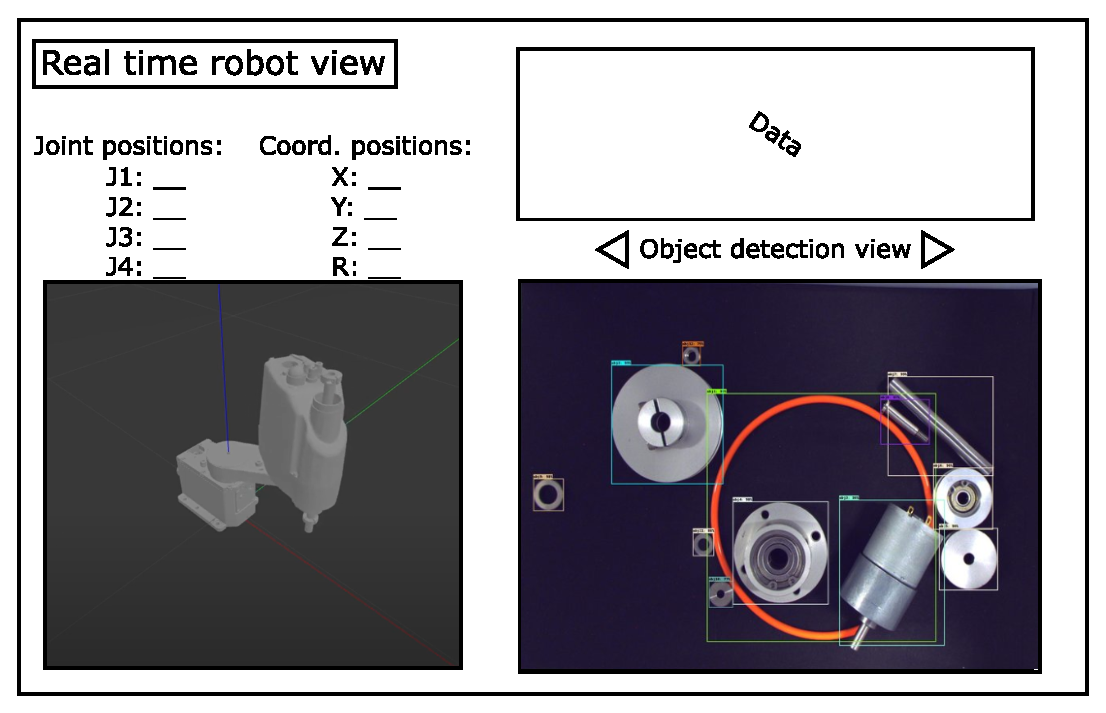
\includegraphics[scale = 0.8]{view_1.eps}
    \caption[]{1. Grafikus rész mockup}
    \vspace{10pt}
    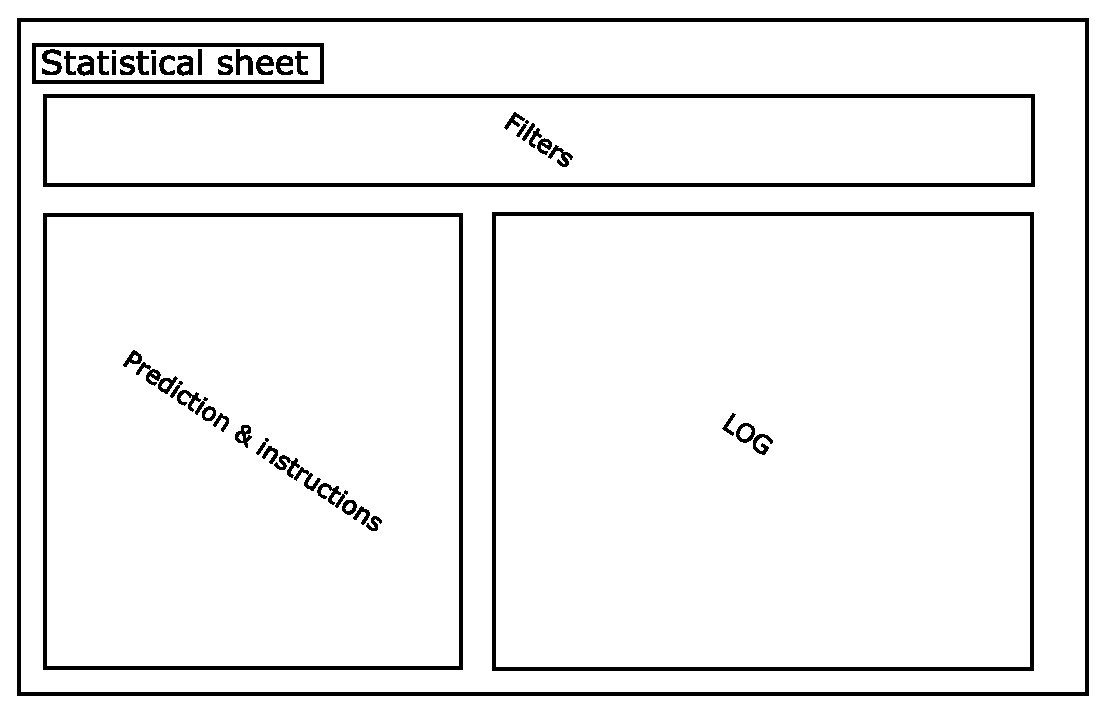
\includegraphics[scale = 0.8]{view_2.eps}
    \caption[]{2. Grafikus rész mockup}
\end{figure}





\end{document}